\chapter{Synthetic Controls}
\label{ch-syn-con}

This chapter is based on Refs.\cite{alves-book}
and \cite{book-mixtape}.

This chapter assumes that
the reader has read Chapter \ref{ch-did}
on the Difference-in-Differences (DID) method.

The Synthetic Controls (SC) method
is a simple enhancement of the DID method.
SC enhances DID in two simple
yet powerful ways:
\begin{enumerate}
\item{\bf Better time resolution.}
DID considers just 2 time snapshots (i.e., a 2-times
time-series)
whereas SC allows
arbitrarily many snapshots (i.e., a time-series with
more than 2 times).
\item{\bf Weighted average of controls.}
DID divides the population
of individuals into just 2 kinds:
the treated and the untreated (aka controls).
SC
divides the 
total population 
into treated and controls
just like DID does, but
it goes further and divides the control population into
multiple subpopulations,
and calculates a weighted average,
called a
``synthetic control",
of those subpopulations.
The weights of the synthetic
control are chosen so that
it mimics as closely as possible
the behavior
of  the treated population for all times
measured before the treatment
was applied.
\end{enumerate}


\begin{figure}[h!]
\centering
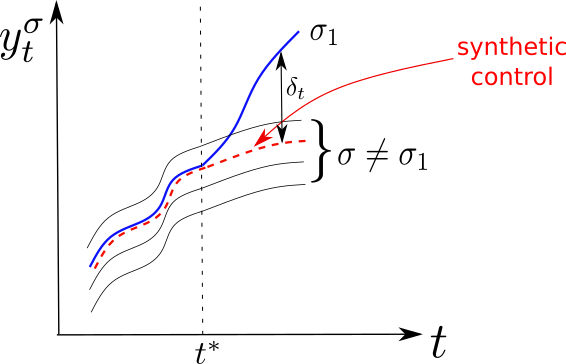
\includegraphics[width=3in]
{syn-con/syn-con-p-lines.png}
\caption{Pictorial
representation of the Synthetic Controls (SC) method.
The outcome $y$ of the synthetic control unit
is colored red and that of the treated unit
is colored blue.
They 
roughly agree for $t<t_*$.
} 
\label{fig-syn-con-p-lines}
\end{figure}

Let us describe these
two enhancements more precisely.

\begin{itemize}
\item{\bf timing}: 
Let $t_k$ for $k=0,1, \ldots, npre-1$
be the pre-treatment times at which
a measurement occurs. Let
$t_k$ for $k=npre, npre+1, \ldots, ntimes-1$
be the post-treatment times
at which a measurement occurs.
Note that
 $npre + npost=ntimes$, and that
$t_*=t_{npre+1}$
is the first measurement time
after the treatment is applied.
$t_0$ is the first measurement time
and $t_{fin}=t_{ntimes-1}$ is
the last one.

\item {\bf subpopulations}:
Let $S_1=\{\s_1\}$ be  the set of treated units
(just one). Let
$S_0 =\{\s:\s\neq \s_1\}$ be the
set of untreated units
 (i.e., controls).
Let $nsam=$ number of 
all units $\s$,
$n_1=|S_1|=1$, and
$n_0= |S_0|=nsam-1$.

\item{\bf weights}:

We want to define a
time-independent weight
$w^\s$ for each unit $\s$
in such a way
that the output $y^\s_t$
for synthetic control
unit behaves like the 
output for the 
treated unit $\s_1$ for $t<t_*$.

Let
\beq
w^{\s_1}=0
\eeq
and

\beq
w^{n_0}=\{ w^\s\}_{\s\neq\s_1}
\;.
\eeq
Define a cost function $\calc$:
 
\beq
\calc(w^{n_0})=
\sum_{t<t_*}
\left(y^{\s_1}_t - \sum_{\s\neq \s_1}
w^\s y^\s_t\right)^2
\eeq
Then calculate $w^{n_0}$
by minimizing the cost function,
subject to the 
constraint that  $w^{n_0}$
be a probability distribution:

\beq
w^{n_0}=
\argmin_{W^{n_0}}
\left\{
\calc(W^{n_0}):
W^\s\geq 0, \sum_{\s\neq \s_1}W^\s =1
\right\}
\;.
\eeq
\end{itemize}
\hrule

Now that we have defined a weight $w^\s$
for every unit $\s$, we can define

\beq
y^\xi_t=
\left\{
\begin{array}{ll}
y_t^{\s_1}&\text{ if } \xi=1
\\
\sum_{\s\neq \s_1}w^\s y_t^\s&\text{ if } \xi=0
\end{array}
\right.
\eeq
and

\beq
\delta_t= y^{\xi=1}_t - y^{\xi=0}_t
\eeq
$\delta_t$
is illustrated
in Fig.\ref{fig-syn-con-p-lines}.
It measures the time dependent
gap (causal effect) between the 
outcome (i.e., $y$)
of the treated unit $\s_1$
and the outcome of the synthetic control unit.

\section{A bnet $G_t$ with weighted 
treatment outcomes}

Our next goal is to
analyze  the SC method using
the formalism of PO theory.
To attain that goal,  
we will first define
in this section a bnet
$G_t$. The bnet $G_t$ 
in this chapter differs
in two important respects from the bnet
$G_t$ defined in Chapter \ref{ch-did}
on the DID method.
First, the $G_t$ in the DID chapter
is defined for only 2 measurement times
whereas the $G_t$ in
this chapter is defined for
 more than 2  measurement times.
Second, the $G_t$ in this chapter 
adds an additional
root node $\rvw$ to
the $G_t$ of the DID chapter.
$\rvw$ acts as a prior to the
treatment outcome node $\rvy_t$.



\begin{figure}[h!]
$$
\begin{array}{ccc}
\xymatrix{
&\rvx^\s\ar[dl]\ar[dr]
\\
\rvd^\s\ar[rr]&
&\rvy_t^\s
}
&&
\xymatrix{
&\rvx\ar[dl]\ar[dr]
\\
\rvd\ar[rr]&
&\rvy_t
\\
&&\rvw\ar[u]
}
\\
\\
G_{t, unit}&&G_t
\end{array}
$$
\caption{$t\in \{t_0, t_1, \ldots, t_{fin}\}$.
The bnet $G_t$ is defined 
by counting units $\s$
for the bnet $G_{t, unit}$. 
} 
\label{fig-syn-con-G}
\end{figure}

 

Suppose $t\in \{t_0, t_1, \ldots, t_{fin}\}$.
For $\xi\in \bool$, define the 
following unit counts:


\beq
N^\xi_{d,y_t,x, w}=
\sum_{\s \in S_\xi}
\indi(d=d^\s, y_t=y_t^\xi,
 x=x^\s, w=w^\s)
\;.
\eeq
Define also

\beq
N_{d,y_t,x, w}=\sum_{\xi\in\bool}
\indi(\xi, d) 
N^\xi_{d,y_t,x, w}
\;.
\eeq

Henceforth,
sums over the subscripts of 
$N_{d,y_t,x, w}$ will
be indicated by a dot.
For example,
$N_{\cdot,y_t,x, w}
=
\sum_d N_{d,y_t,x, w}
$.

The TPMs,
printed in blue,
for the 
bnet
$G_t$
shown
in Fig.\ref{fig-syn-con-G},
are as follows.


\beq\color{blue}
P_{\rvx}(x)=  \frac{N_{\cdot,\cdot,x, \cdot}}
{N_{\cdot, \cdot, \cdot, \cdot}}
\eeq
 
\beq\color{blue}
P_{\rvd|\rvx}(d|x)= \frac{N_{d,\cdot,x, \cdot}}
{N_{\cdot, \cdot, x, \cdot}}
\eeq

\beq\color{blue}
P_{\rvy_t|\rvd, \rvx, \rvw}(y_t|d,x, w)=
\frac{N_{d,y_t,x,w}}{N_{d,\cdot,x,w}}
\eeq

\beq\color{blue}
P_{\rvw}(w)=  \frac{N_{\cdot,\cdot,\cdot, w}}
{N_{\cdot, \cdot, \cdot, \cdot}}
\eeq

\section{PO analysis}
In this section,
we show how
to analyze the
DID method
using the formalism of PO theory.



\begin{figure}[h!]
$$
\begin{array}{ccccc}
\xymatrix{
&\rvx\ar[dl]\ar[dr]
\\
\rvd\ar[rr]&&\rvy_t
\\
&&\rvw\ar[u]
}
&&
\xymatrix{
&\rvx\ar[dl]\ar[dr]
\\
\rvd=d&\rvtd=\td\ar[r]&\rvy_t
\\
&&\rvw\ar[u]
}
\\
\\
G_t&&G_{t, im}
\end{array}
$$
\caption{$t\in \{t_0, t_1, \ldots, 
t_{fin}\}$.
Bnet 
$G_{t, im}= \kappa_{\rvd\rarrow\rvy_t}
(\td)G_t$
is obtained by applying 
the imagine operator to arrow 
$\rvd\rarrow\rvy_t$
of bnet $G_t$.}
\label{fig-syn-con-G-im}
\end{figure}

As usual for PO theory,
we will consider
expected values of $y^\s_t$:


\beq
E_{\s|d,\td, x}[y^\s_t(\td^\s, x^\s)]=
 E_{y_t|d, \td, x}[\rvy_t(\td, x)]=
\caly_{d|\td, x}(t)
\eeq

To calculate these
expected values, we need a ``model"
with probability 
distributions.
In this case,
the needed model and probability
distributions are
provided by the
bnets depicted in Fig.\ref{fig-syn-con-G-im}.
The TPMs,
printed in blue,
for the 
 bnet
$G_{t, im}$
in Fig.\ref{fig-syn-con-G-im},
are as follows.
Note
that the
TPMs for the bnet $G_{t, im}$
are defined in 
terms
of the TPMs for the bnet $G_t$.



\beq\color{blue}
P(x)=P_{\rvx}(x)
\eeq

\beq\color{blue}
P(d|x)= 
P_{\rvd|\rvx}(d|x)
\eeq
 
\beq\color{blue}
P(y_t|\td, x,w)=
P_{\rvy_t|\rvt, \rvx, w}
(y_t|\td, x, w)
\eeq

\beq\color{blue}
P((\td)')=\delta(
(\td)', \td)
\eeq

\beq\color{blue}
P(w)=P_{\rvw}(w)
\eeq

\begin{figure}[h!]
\centering
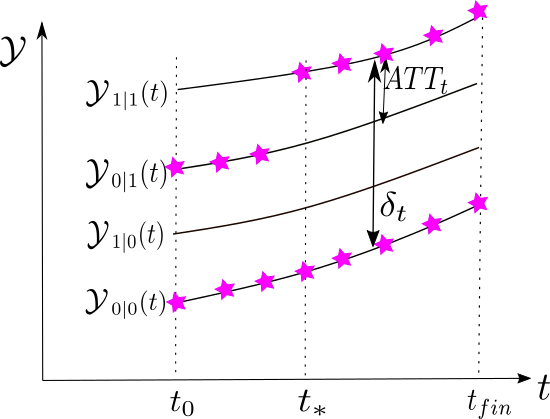
\includegraphics[width=3in]
{syn-con/syn-con-bc.png}
\caption{Four different time-dependent
expected 
values $\caly_{d|\td}(t)$ of $y^\s_t$
for bnet $G_{t, im}$
The $2*ntimes$ magenta  stars
represents the $2*ntimes$ DID measurements.} 
\label{fig-syn-con-bc}
\end{figure}

Henceforth, 
for simplicity, we will
omit the confounder state $x$
from the indices of $\caly$; i.e., we will write
$\caly_{d|\td}(t)$
instead of $\caly_{d|\td, x}(t)$.
The fact that we will
not explicitly
mention $x$ does not
mean that it doesn't exist
or that it doesn't affect our analysis.
If there are confounders,
they cannot be neglected.
As discussed in Chapter \ref{ch-po}
under the subject of strata-matching in PO,
one must condition $\caly$
on a single $x$ stratum
and, later on,  one must average
over all the possible $x$ strata.


Let $\calm\caly_{d|\td}(t)$ denote the
{\bf measured $\caly_{d|\td}(t)$}.
We define this quantity as

\beq
\calm\caly_{d|\td}(t)
=
\caly_{d|\td}(t)
\left[ \indi(d=0, t< t_*)+
\indi(d=\td, t> t_*)\right]
\eeq
Now we claim that the DID 
$\delta_t$ calculated in the 
previous section 
can be expressed in PO formalism as follows:

\beqa
\delta_t=
\caly_{1|1}(t)-\caly_{0|0}(t)=SDO_t
\;
\eeqa
for $t\geq t_*$.
Fig.\ref{fig-syn-con-bc}
depicts the
four functions
$\caly_{d|\td}(t)$
for $t$ in the interval  $[t_0, t_{fin}]$
and for $d,\td\in \bool$.
The $\caly$ coordinates
of the $2*ntimes$ magenta stars in 
Fig.\ref{fig-syn-con-bc} can 
be calculated using bnet $G_t$.
Note that in Fig.\ref{fig-syn-con-bc},
we display a large gap
between the curve $\caly_{0|\td}(t)$
for $\td\in \bool$.
In reality, the priors
$\rvw$ have been
calculated so as to make that
gap as small as possible.
Hence, to a good approximation,

\beq
\delta_t\approx ATT_t
\eeq
Hence, unlike in the DID method,
in the SC method, to a good(?)
approximation, we don't have to worry
about parallel trends.